\chapter{Toolfindung}
\label{ch:toolfindung}

In diesem Kapitel werden vier Tools untersucht, welche \gls{ub} auffinden sollen:
\begin{itemize}
  \item PC-lint Plus \cite{misc:pclintplus}
  \item Cppcheck \cite{misc:cppcheck}
  \item \gls{ubsan} (wird von GCC und Clang++ verwendet) \cite{misc:ubsan}
  \item PVS-Studio \cite{misc:pvsstudio}
\end{itemize}
Die Tools werden dabei anhand einer Bewertungsmatrix mit den Anforderungen F-1 bis F-7 und NF-1 und NF-3 bewertet. Die Anforderungen sind mit Zahlen von eins bis fünf gewichtet, wobei
eine höhere Zahl für eine höhere Relevanz steht.
\begin{figure}[htpb]
  \centering
  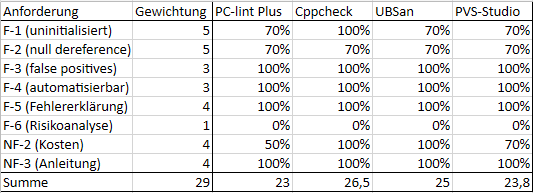
\includegraphics[width=0.8\textwidth]{toolfindung}
  \caption{Bewertungsmatrix}
  \label{img:toolfindung}
\end{figure}

Die Erfüllung der Anforderungen F-1 und F-2 wird in \ref{sec:codeanalyse} beschrieben. \newline
Da jedes Tool von der Kommandozeile aus bedienbar ist, sind alle Tools automatisierbar. Dies ermöglicht auch eine Integration in Projekte jeder Art. Für PVS-Studio existiert jedoch
zusätzlich eine Extension für Visual Studio \cite{misc:pvsplugin}. \newline
Eine Risikoanalyse wird von keinem Tool zur Verfügung gestellt. \newline
Im Gegensatz dazu verfügt jedes Tool über eine Dokumentation. Beim Aufruf am 02.02.2021 referenzierte die Dokumentation von PVS-Studio (\cite{misc:pvsdoku}) nicht mehr vorhandene Seiten. Zusätzlich
funktionierte die integrierte Suchfunktion nicht mit einzelnen Wörtern. Dies ist aktuell (letzter Aufruf 16.06.2021) nicht mehr der Fall.\newline
Sowohl Cppcheck als auch \gls{ubsan} sind kostenfrei verfügbar. \newline
PVS-Studio kostet im ersten Jahr, für ein Entwicklerteam mit 10-30 Entwicklern, 21.000€. Für jedes folgende Jahr belaufen sich die Kosten auf 80\% des Preises (16.800€).\newline
Die zuständigen Stelle von PC-Lint Plus hat bezüglich auf eine Preisanfrage, zum aktuellen Zeitpunkt, noch keine Rückmeldung gegeben. Aus diesem Grund wird NF-2 bei diesem Tool
vorläufig mit 50\% bewertet.

\section{Codeanalyse}
\label{sec:codeanalyse}

\subsection{PVS-Studio}

\begin{figure}[htpb]
  \centering
  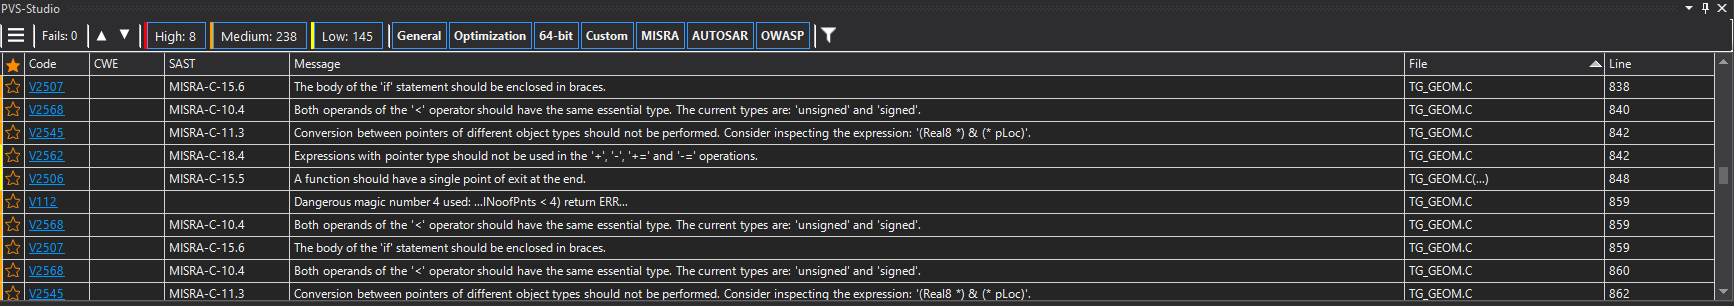
\includegraphics[width=1\textwidth]{pvs-tg-geom}
  \caption{Ausschnitt der von PVS-Studio gemeldeten Fehler}
  \label{img:pvs-tg-geom}
\end{figure}

Die Extension von PVS-Studio für Visual Studio kann circa 600 verschiedene Fehler erkennen und mit einer kurzen Beschreibung ausgeben. Es kann dabei frei ausgewählt werden, welche Arten von
Fehlern gemeldet werden sollen. \newline
Wird nur die Datei \glqq{}TG\_GEOM.C\grqq{} analysiert, so gibt das Tool insgesamt 361 Fehlermeldungen in der Datei aus. Die Fehler werden dabei in die Kategorien \glqq{}High\grqq{}
(0 Fehler), \glqq{}Medium\grqq{} (227 Fehler) und \glqq{}Low\grqq{} (134 Fehler) eingestuft. Zusätzlich in \ref{img:pvs-tg-geom} gemeldete Fehler stammen aus anderen Dateien.

PVS-Studio erkennt keine uninitialisierten Variablen in der analysierten Datei, obwohl dies beispeilsweise in Zeile 992 der Fall ist. Eine erste Annahme, dass dies geschieht, weil die
Variablen nicht direkt ausgewertet werden, sondern über verschiedene Dateien in verschiedenen Funktionen aufgerufen werden, wurde wiederlegt. Auch eine Analyse der gesamten Solution
ergab keinen Fehler, welcher sich mit uninitialisierten variablen beschäftigt. \newline
Im Kontrast dazu erkennt PVS-Studio alle erwarteten Fehler im Code-Beispiel \ref{subsec:indeterminate}. Durch eine Integration, und erfolgreiche Fehlererkennung, des Beispiel-Codes in
\glqq{}TG\_GEOM.C\grqq{} wurde widerlegt, dass PVS-Studio mit der Menge an Code überfordert ist. \newline
PVS-Studio erkennt nicht initialisierte Variablen erfolgreich in dem Code-Beispiel. In \glqq{}TG\_GEOM.C\grqq{} werden allerdings keine uninitialisierten Variablen gefunden. Dafür
werden zahlreiche andere Fehler markiert. PVS-Studio erhält somit für F-1 eine Bewertung von 65\%. 50\% für eine korrekte Fehlererkennung im Beispielcode und 15\% für eine allgemein
sehr gute Fehlererkennung.

PVS-Studio markiert den in \ref{subsec:nullpointer} beschriebenen Code erfolgreich als fehlerhaft und erkennt fehlerhafte Benutzung von Pointern beispielsweise in
\glqq{}CryptoPP/algparam.h\grqq{} Zeile 36. Somit bekommt das Tool eine Wertung von 80\% für F-2. 20\% werden abgezogen, da keine explizite Nullpointerdereferenzierung
aufgezeigt wurde.

Anmerkung: Die Analysezeit für die gesamte Solution betrug circa eine Minute. \newline
Alle weiteren Tools werden unter den gleichen Bedienungen, wie PVS-Studio getestet.

\subsection{Cppcheck}

\begin{figure}[htpb]
  \centering
  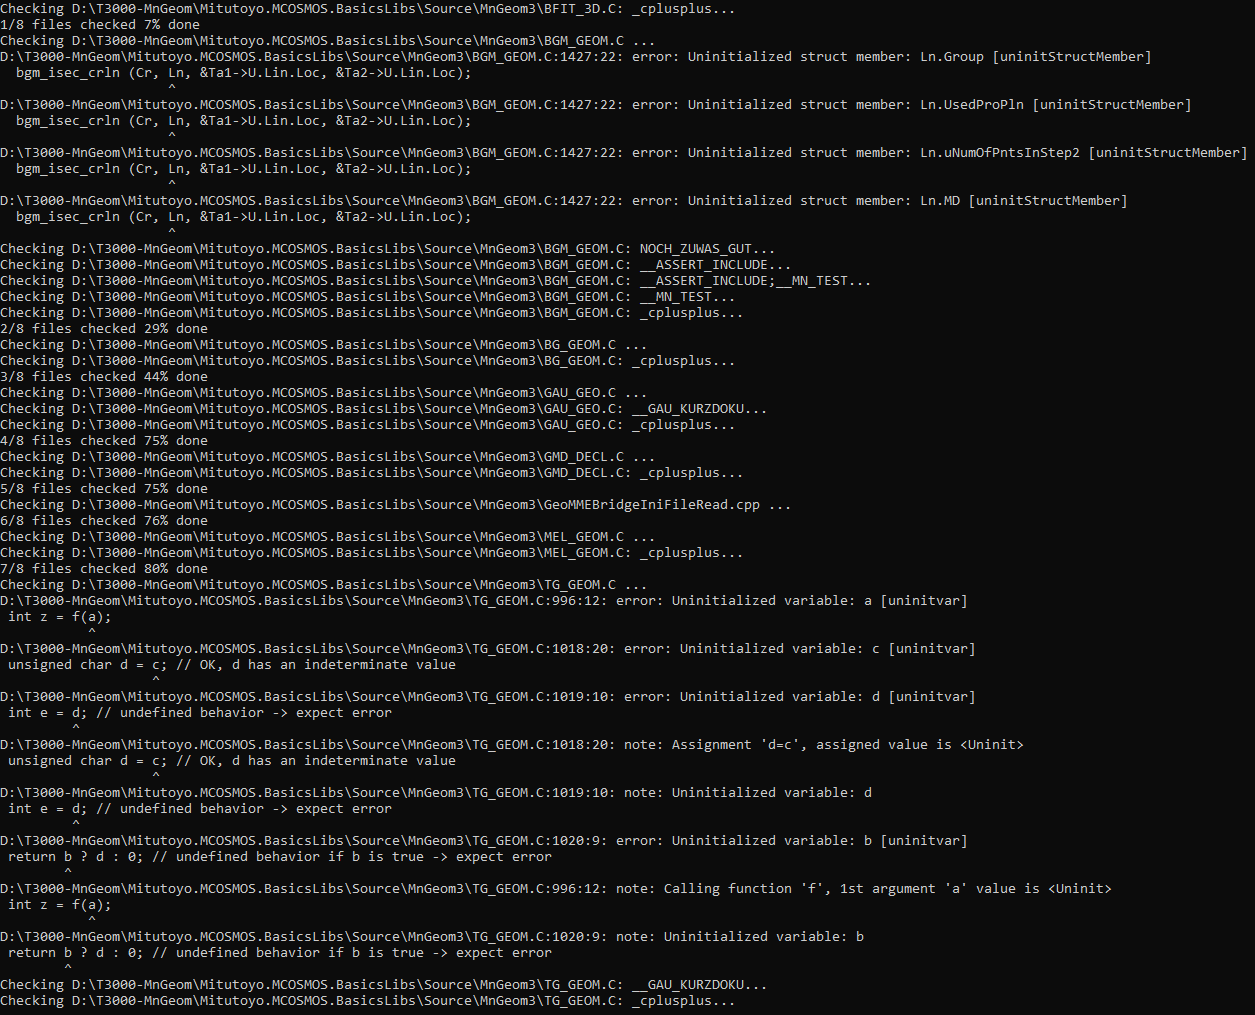
\includegraphics[width=1\textwidth]{cppcheck-mngeom}
  \caption{Von Cppcheck im Ordner MnGeom3 erkannte Fehler}
  \label{img:cppcheck-mngeom}
\end{figure}

Im Ordner \glqq{}MnGeom3\grqq{} erkennt Cppcheck die in \glqq{}TG\_GEOM.C\grqq{} vorhandenen Test-Fehler und zusätzlich uninitialisierte Variablen in \glqq{}BGM\_GEOM.C\grqq{}. Letztere
sind zu Beginn nicht initialisiert, zum Zeitpunkt, an welchem Cppcheck diese als Fehler markiert, sind die Variablen allerdings initialisiert. \newline

Cppcheck erkennt Nullpointerderefernzierung im Code-Beispiel \ref{subsec:nullpointer}, auch in der Solution von MBasicLibs werden beispielsweise in \glqq{}CryptoPP/algparam.h\grqq{}
mehrere Nullpointerdereferenzierungen markiert.

Für F-1 erhält Cppcheck 45\%. 50\% für eine korrekte Fehlererkennung im Beispiel-Code und -5\% für false positives. \newline
Für F-2 erhält Cppcheck 75\%. 50\% für eine korrekte Fehlererkennung im Beispiel-Code und 25\% für das Erkennen von Nullpointerderefernzierungn in MBasicLibs. Dort wurden allerdings
jedes Auftreten des Schlüsselworts \textit{NULL} als Nullpointerdereferenzierung markiert. Deshalb keine 100\%.

Anmerkung: Cppcheck benötigte für die Analyse der Solution circa 6 Minuten.

\subsection{UBSan}

Das Folgen einer von Clang geschriebenen Anleitung (erreichbar unter \cite{misc:ubsan}) ,zur Installation und Anwendung von UBSan, verlief erfolglos. Somit beruhen alle in \ref{img:toolfindung} 
beschriebenen Werte zu UBSan auf Informationen aus der Dokumentation von Clang und GCC, sowie Erfahrungsberichten aus dem Internet. Diese Quellen sind minderwertiger als eine 
Überprüfung des Tools anhand einer Analyse von MBasicLibs. Allerdings ist das Tool kostenlos und sollte somit immer in Betracht gezogen werden. 

F-1 und F-2 werden aufgrund der Dokumentation (\cite{misc:ubsan}) vorläufig mit 50\% bewertet. \newline
F-3 bis F-5 sollten laut der Dokumentation mit 100\% gewertet werden. Aus den Erfahrungen mit den anderen vorgestellten Tools wird allerdings bei F-3 20\% abgezogen, solange nicht das 
Gegenteil bewiesen wird. \newline
Da die Anleitung nicht sehr ausführlich ist und keine Aufschlüsse über von UBSan ausgegebenen Fehler-Nachrichten hat, werden bei NF-3 40\% abgezogen.

\subsection{PC-Lint Plus}

\begin{figure}[htpb]
  \centering
  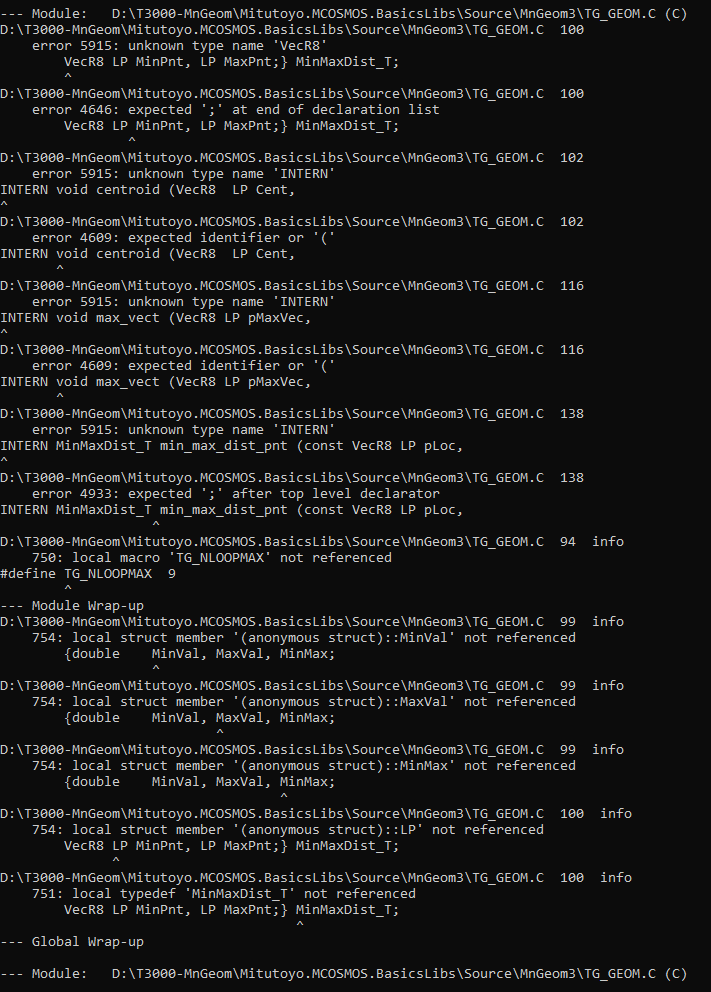
\includegraphics[width=1\textwidth]{pclint-analysis}
  \caption{Von PC-Lint Plus in TG\_GEOM.C gefundene Fehler}
  \label{img:pclint-analysis}
\end{figure}

PC-Lint Plus fand in \glqq{}TG\_GEOM.C\grqq{} nur von Mitutoyo CTL eingeführte Variablen (oder ähnliches) und markierte diese als Fehler (vgl. \ref{img:pclint-analysis}). Der darin vorhandene Beispiel-Code 
wurde nicht als fehlerhaft markiert. Allerdings wurde der Beispiel-Code korrekt markiert, wenn dieser als separate Datei von PC-Lint Plus ausgewertet wurde.

PC-Lint Plus erkannte keine Nullpointerdereferenzierung in MBasicLibs, eine separate Datei mit Beispiel-Code wurde erfolgreich erkannt.

Für F-1 erhält PC-Lint Plus 40\% .50\% für eine korrekte Fehlererkennung im Beispiel-Code und -10\% dafür, dass nur korrekter Code in \glqq{}TG\_GEOM.C\grqq{} als fehlerhaft markiert 
wurde. \newline
Für F-1 erhält Cppcheck 50\%. 50\% für eine korrekte Fehlererkennung im Beispiel-Code und 0\% für keine erkannten Pointer-Fehler in \glqq{}TG\_GEOM.C\grqq{}.

Anmerkung: PC-Lint Plus benötigte für die Analyse der Solution circa 4 Minuten.

\section{Auswahl}
\label{sec:auswahl}

PVS-Studio erreicht in der Bewertungsmatrix (Abbildung: \ref{img:toolfindung}) die höchste Punktzahl und ist somit Sieger der Bewertung und daraus resultierend die Toolempfehlung.

Kritikpunkte an PVS-Studio sind der hohe Preis und eine allgemein geringe Bekanntheit. Dies wird aber durch eine Integration in Visual Studio, und der damit verbundenen mit Abstand 
besten User Experience, ausgeglichen. Cppcheck bietet auch eine grafische Oberfläche an, diese ist allerings nicht so umfangreich und nicht in Visual Studio integriert. \newline
Zusätzliche bieten sowohl PVS-Studio, als PC-Lint Plus einen Kundenservice an, welchen die kostenlosen Tools nicht besitzen. Dieser Kundenservice wirkt auch dem Mangel an Hilfestellungen 
durch andere Entwickler entgegen, welchen PVS-Studio aufgrund der bereits erwähnten geringen Bekanntheit aufweist. \newline
Zusätzlich können die kostenfreien Tools ergänzend zu dem schlussendlich ausgewählten Tool eingesetzt werden. Dies ermöglicht eine höhere Fehlerabdeckung, garantiert allerdings nicht,
dass neue, beziehungsweise mehr, Fehler erkannt werden. Da das Einsetzen der kostenlosen Tools nur Zeit kostet, ist der Einsatz dieser immer eine Überlegung wert.